\section{Un petit mot historique}
\textbf{Cantor} (1845-1918): théorie des ensembles de nombres réels;
tout intervalle de $\mathbb{R}$ est non-dénombrable.

\textbf{Borel} (1871-1956): théorie de la mesure; tout intervalle
de $\mathbb{R}$ est de mesure non nulle; notion de propriété vraie
presque partout: une propriété $P$ est vraie presque partout si
elle est vérifiée l'ensemble complet hormis un sous-ensemble de mesure
nulle.

\textbf{Baire} (1874-1932): point de vue topologique; tout intervalle
n'est pas de première catégorie; une propriété $P$ est dite
vraie presque partout au sens de Baire si elle est vérifiée sur tout
l'ensemble hormis un sous-ensemble de première catégorie.

\section{Définitions}

Soit $(X, \mathcal{T})$ un espace topologique (fixé tout au long de cette
section).

\begin{df}
  Un sous-ensemble $A$ de $X$ est dit nulle part dense s'il vérifie
  $$\mathrm{int}\left(\mathrm{adh}(A)\right) = \varnothing.$$

  De manière équivalente, $A$ est dit nulle part dense si le complémentaire
  de son adhérence est dense dans $X$.
\end{df}

Par exemple, dans $\mathbb{R}$ muni de sa topologie usuelle, l'ensemble
vide, les singletons, l'ensemble des nombres naturels et l'ensemble des
nombres entiers sont tous nulle part denses.

\begin{prop}
  L'ensemble des parties nulle part denses de $X$ est héréditaire et
  est stable par union finie  et par fermeture.
\end{prop}

\begin{rem}
  Montrer qu'un sous-ensemble $C$ de $X$ est dense revient à
  montrer que $\mathrm{adh}(C) = X$, c'est-à-dire
  $\forall x\in X$, $\forall O_x\in\mathcal{T}$ , $x\in O_x\implies O_x\cap C\neq
  \varnothing$.

  Cela revient au même que de montrer que tout ouvert $O$ de $X$ non vide,
  $O\cap C\neq \varnothing$.
\end{rem}

\begin{proof}
  Il est clair que cette classe est stable par fermeture. L'hérédité est
  facile à démontrer étant donné que le passage à l'intérieur et à l'adhérence
  préservent les inclusions.

  Il reste donc à montrer que cette classe est stable par union finie.
  Il suffit de le montrer pour deux ensembles (et d'itérer lorsque plus de
  deux ensembles interviennent)

  Soient
  $A$, $B$ deux sous-ensembles nulle part denses de $X$. Alors le complémentaire
  de l'adhérence de $A$ est dense dans $X$, c'est-à-dire pour tout ouvert $O$ non vide
  de $\mathcal{T}$, $O\cap (X\setminus \mathrm{adh(A)})$ est non vide. De même
  pour le complémentaire de l'adhérence de $B$.

  On doit montrer que le complémentaire de l'adhérence de $A\cup B$ est dense
  dans $X$. L'adhérence de $A\cup B$ correspondant à l'union des adhérences,
  on doit donc montrer que (en appliquant les lois de De Morgan):
  $$\forall O \in \mathcal{T}, O\neq \varnothing\implies
  O \cap (X\setminus \mathrm{adh}(A))\cap (X\setminus \mathrm{adh}(B))\neq\varnothing$$
  Soit $O$ un ouvert de $X$.
  Puisque le complémentaire de l'adhérence de $A$ est un ouvert dense,
  $O\cap (X\setminus \mathrm{adh}(A))$ est un ouvert non vide. Puisque
  le complémentaire de l'adhérence de $B$ est dense, on a le résultat.
\end{proof}

Toutefois la classe des ensembles nulle part denses n'est pas stable par union
dénombrable. On introduit donc la notion d'ensemble de première catégorie:

\begin{df}
  Un sous-ensemble $A$ de $X$ est dit de première catégorie s'il s'agit d'une
  union dénombrable de parties nulle part denses.
\end{df}

Par exemple, dans $\mathbb{R}$ muni de sa topologie usuelle, l'ensemble
des nombres rationnels est de première catégorie (il s'agit d'une union
dénombrable de singletons) mais n'est pas nulle part dense car son
adhérence étant $\mathbb{R}$, l'intérieur de son adhérence est non vide.

En particulier, ceci montre que l'ensemble des parties de première
catégorie de $X$ n'est pas stable par fermeture en général, en admettant
que $\mathbb{R}$ n'est pas de première catégorie (pour sa topologie usuelle).
En plus, il s'agit d'un exemple de sous-ensemble de première catégorie qui
n'est pas nulle part dense.

\begin{prop}
  Le sous-ensemble des parties de première catégorie de $X$ est héréditaire
  et stable par union dénombrable.
\end{prop}

\begin{proof}
  L'hérédité est claire. Une union dénombrable d'unions dénombrables d'ensembles
  nulle part denses étant une union dénombrable d'ensembles nulle part denses,
  l'autre partie du résultat est claire.
\end{proof}

La dernière définition introduite ici est celle de la propriété de Baire.
\begin{df}[Propriété de Baire]
  On dit que $X$ a la propriété de Baire si toute intersection dénombrable
  d'ouverts denses de $X$ est dense dans $X$. Dans ce cas on dit que $X$
  est un espace de Baire.
\end{df}

Insistons sur l'importance de la dénombrabilité de l'intersection considérée.
On montre plus
tard que $\mathbb{R}$ muni de sa topologie usuelle est un espace
de Baire. Considérons l'intersection non dénombrable d'ouverts denses
$\bigcap_{r\in\mathbb{R}}\mathbb{R}\setminus \{r\}$. Elle est vide
donc non dense dans $\mathbb{R}$.

\textbf{Remarque}: pour rappel, une intersection infinie d'ouverts n'est
pas ouverte en général. Il est en de même pour une intersection d'ouverts
denses dans $X$; si $X$ a la propriété de Baire, leur intersection
sera dense dans $X$ mais ne sera pas nécessairement ouverte.
Essayez d'expliciter un exemple à titre d'exercice.

\section{Formulations équivalentes}
Soit $(X, \mathcal{T})$ un espace topologique fixé.

La propriété de Baire peut être exprimée de manière équivalente
en termes de fermés:
\begin{prop}
  $X$ a la propriété de Baire \ssi{} toute union dénombrable de fermés
  d'intérieur vide est d'intérieur vide.
\end{prop}

\textbf{Remarque}: une union de fermés n'est pas nécessairement
un fermé. Vous êtes invités à produire un exemple de famille
dénombrable de fermés d'intérieur vide tel que leur union n'est
pas fermée.

\begin{proof}
  Supposons que $X$ a la propriété de Baire. Soit $(F_n)_{n\in\mathbb{N}}$ une
  famille de fermés de $X$ d'intérieur vide. Alors la famille
  $(X\setminus F_n)_{n\in\mathbb{N}}$ est une famille d'ouverts denses dans $X$
  (car l'adhérence du complémentaire d'un ensemble correspond au complémentaire
  de son intérieur). Par la propriété de Baire,
  $$X\setminus\mathrm{int} \left(\bigcup_{n\in\mathbb{N}} F_n \right)
  =\mathrm{adh}\left(\bigcap_{n\in\mathbb{N}} X\setminus F_n\right) = X$$
  En passant au complémentaire, on a la première implication.

  L'autre implication se démontre de manière similaire et est donc laissée
  à titre d'exercice.
\end{proof}

On peut également énoncer la propriété de Baire en termes d'ensembles
résiduels. Introduisons les:
\begin{df}
  Un sous-ensemble $A$ de $X$ est dit résiduel si son complémentaire
  est de première catégorie.
\end{df}

\begin{prop}
  $X$ a la propriété de Baire \ssi{}  tout
  ensemble résiduel est dense dans $X$.
\end{prop}

\begin{proof}
  Supposons que $X$ est un espace de Baire. Soit $A$ un ensemble résiduel,
  c'est-à-dire $X\setminus A = \bigcup_{n\in\mathbb N} S_n$ où les $S_n$ sont
  des sous-ensembles de $X$ nulle part denses. Alors chaque fermeture de $S_n$
  est un sous-ensemble de $X$ d'intérieur vide. Par la propriété de Baire,
  $$\mathrm{int}(X\setminus A) =
  \mathrm{int}\left(\bigcup_{n\in\mathbb N}S_n\right)\subseteq
  \mathrm{int}\left(\bigcup_{n\in\mathbb N}\mathrm{adh}(S_n)\right)
  \overset{\mbox{Baire}}{=} \varnothing$$
  En passant au complémentaire, on déduit que l'adhérence de $A$ est $X$,
  c'est-à-dire $A$ est dense dans $X$.

  Réciproquement, supposons que tout ensemble résiduel est dense dans $X$.
  Soit $(F_n)_{n\in\mathbb N}$ une famille de fermés d'intérieur vide. Alors
  il s'agit d'une famille de sous-ensembles nulle part denses de $X$, donc
  le complémentaire de leur union est dense dans $X$ (car il s'agit d'un
  ensemble résiduel). Ceci implique que l'intérieur de l'union des $F_n$
  est vide, ce qu'on voulait montrer.
\end{proof}


\section{Théorème de Baire}
Le théorème de Baire affirme que les espaces métriques complets
sont des espaces de Baire, ce qui nous fournira des exemples
concrets d'espaces de Baire.

\begin{thm}[Théorème de Baire]
  Soit $(X, d)$ un espace métrique. Si $X$ est complet, alors
  il a la propriété de Baire.
\end{thm}

\begin{proof}
  Soit $(O_n)_{n\in\mathbb{N}}$ une famille dénombrable d'ouverts denses
  dans $X$. Montrons que tout ouvert de $X$ a une intersection non vide
  avec $\bigcap_{n\in\mathbb{N}}O_n$. Soit $U$ un ouvert de $X$.

  Puisque $O_0$ est un ouvert dense dans $X$, il existe $x_0$ dans
  $O_0\cap U$. Il existe $r_0 \in \left]0, 1\right]$ tel
  que $B[x_0, r_0]\subseteq  O_0\cap U$\footnote{La notation
    $B[y, r]$ est une notation pour dénoter la boule
    fermée de centre $y$ et de rayon $r$. Pour rappel, dans un espace
    métrique, l'adhérence de la boule ouverte ne correspond pas nécessairement
    à la boule fermée; on a toujours $\mathrm{adh}(B(y, r))\subseteq B[y, r]$.}.
  De même, puisque $O_1$ est dense dans $X$, il existe $x_1$ dans
  $O_1\cap B(x_0, r_0)$, et $r_1\in\left]0, 2^{-1}\right]$ tels que
  $B[x_1, r_1]\subseteq O_1\cap B(x_0, r_0)$.

  En itérant de la sorte, on construit deux suites $(x_n)_{n\in\mathbb{N}}$
  et $(r_n)_{n\in\mathbb{N}}$ telles que $x_n\in O_n\cap B(x_{n-1}, r_{n-1})$,
  ${B}[x_n, r_n]\subseteq O_n$
  et $r_n\in\left]0, 2 ^{-n}\right]$. La suite $(x_n)_{n\in\mathbb{N}}$ ainsi
  construite est de Cauchy dans un espace métrique complet; elle converge
  donc vers un élément $x$ de $X$.

  Par la première étape, on a $(x_n)_{n\in\mathbb{N}}\subseteq {B}[x_0, r_0]$
  qui est un sous-ensemble de $U$. Ceci montre que $x$ est élément de $U$
  (puisqu'une boule fermée est fermée).

  Pour tous naturels $n$ et $p$, on a par construction $x_{n+p}\in
  {B}[x_n, r_n]$ et en faisant tendre $p$ vers l'infini, étant
  donné que $B[x_n, r_n]$ est fermée, on en déduit que $x$
  est un élément de $B[x_n, r_n]$ qui est contenue dans $O_n$,
  ce qui prouve que $x$ est bien dans l'intersection des $O_n$.
\end{proof}

Un autre résultat repris comme faisant partie du théorème de Baire concerne
la topologie induite.
\begin{thm}\label{baire:ind}
  Soient $(X, \mathcal{T})$ un espace de Baire et $O$ un ouvert de $X$.
  $O$ muni de la topologie induite est également un espace de Baire.
\end{thm}

\begin{rem}[Rappels]
  Soit $(X, \mathcal{T})$ un espace topologique.
  Rappelons que si $B$ est un sous-ensemble de $X$, la topologie
  induite sur $B$ est la topologie $\mathcal{T}_B$ suivante:
  $$\mathcal{T}_B=\left\{U\cap B\mid U\in\mathcal{T}\right\}.$$
  De plus, si on note $\mathcal{F}$ l'ensemble des fermés de $X$,
  on a la caractérisation suivante des fermés de la topologie
  induite:
  $$\mathcal{F}_B=\left\{F\cap B\mid F\in\mathcal{F}\right\}.$$

  \textbf{Propriété}: la fermeture de $A$ au sens de $\mathcal T_B$ correspond
  l'intersection de $B$ et de la fermeture de $A$ au sens
  de $\mathcal T$ (car on regarde le plus petit fermé contenant $A$).

  \begin{proof}
    Soit $F\in\mathcal F_B$ contenant $A$. Alors $F = G\cap B$ pour un
    fermé $G\in\mathcal F$. Puisque $ A \subseteq F\subseteq G$, $G$
    contient l'adhérence de $A$ au sens de $X$ (qui est le plus petit
    fermé de $X$ contenant $A$), donc $F$ contient $\mathrm{adh}_X(A)\cap B$.
    Ceci montre que le plus petit fermé de $B$ contenant $A$
    est $\mathrm{adh}_X(A)\cap B$, ce qu'on voulait montrer.
\end{proof}

  \textbf{Propriété}: si on suppose que $B$ est ouvert, alors l'intérieur d'un
  sous-ensemble $A$ de $B$ au sens de $\mathcal T_B$ correspond à
  son intérieur au sens de $\mathcal T$
  (car les ouverts de la topologie induite sur $B$ sont des
  ouverts de $X$).

  \begin{proof}
    Soit $U\subseteq A$ un ouvert de $B$. Alors $U$ est un
    ouvert de $X$ (car il est l'intersection de $B$ qui est ouvert
    et d'un ouvert de $X$). Donc $U$ est contenu dans l'intérieur
    de $A$ au sens de $X$. Puisque l'intérieur de $A$ est un sous-ensemble
    de $A$, il s'agit d'un ouvert de $B$ (car $B$ est ouvert),
    et donc du plus grand
    ouvert de $B$ contenu dans $A$, ce qu'on voulait montrer.
    \end{proof}
\end{rem}

Nous rappelons un résultat vu l'année passée qui servira dans la preuve
d'un lemme intermédiaire.
\begin{lem}\label{rap:top1}
  Soient $(X, \mathcal{T})$ un espace topologique, $U$ et $O$ deux ouverts
  de $X$. Si $U$ et $O$ sont disjoints, alors l'adhérence de $U$ est
  disjointe de $O$.
\end{lem}
% Figure pour illustrer que si deux ouverts sont disjoints, alors
% l'adhérence du premier est disjoint du second ouvert
\begin{figure}[!h]
  \begin{center}
    \caption{Illustration du lemme \ref{rap:top1}}%
    \label{fig:ouv_disjoints}
    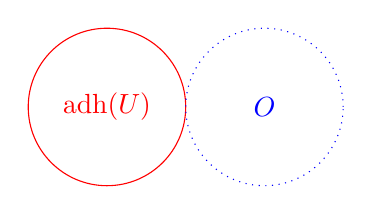
\begin{tikzpicture}
      \draw [red] (0 , 1) ellipse (1 cm and 1 cm) node {$\mathrm{adh}(U)$};
      \draw [blue, dotted] (2 , 1) ellipse (1 cm and 1 cm) node {$O$};
    \end{tikzpicture}
\end{center}
\end{figure}

\begin{proof}
  Supposons qu'il existe $x$ un élement de $\mathrm{adh}(U)\cap O$.
  Alors pour tout voisinage $V$ de $x$, $V$ intersecte $U$ puisque
  $x$ est dans l'adhérence de $U$. Or $O$ est un voisinage de $x$
  donc son intersection avec $U$ doit être non vide. Cela constituant
  une contradiction, on conclut que $\mathrm{adh}(U)\cap O$ est vide.
\end{proof}


Pour prouver le théorème \ref{baire:ind},
on introduit tout d'abord un lemme utile
à sa preuve.
\begin{lem}\label{baire:ind:help}
  Soient $(X, \mathcal{T})$ un espace de Baire et $O$ un ouvert de $X$.
  Un sous-ensemble $A$ nulle part dense de $O$ (au sens de la topologie
  induite) est nulle part dense dans $X$ (au sens de $\mathcal{T}$).
\end{lem}

\begin{proof}
  Montrer que $A$ est nulle part dense revient à montrer que
  tout ouvert compris dans l'adhérence de $A$ (au sens de $X$) est vide. Soit $U$
  un ouvert de $X$ tel que $U$ est contenu dans l'adhérence
  de $A$. Alors $U\cap O$ est contenu dans $\mathrm{adh}_O(A) =
  \mathrm{adh}_X(A)\cap O$, d'intérieur vide, ce qui implique que $U$ et $O$
  sont disjoints.

  Par le lemme \ref{rap:top1}, $U\cap \mathrm{adh}_X(O)$
  est également vide, or on a la chaîne d'inclusions suivante:
  $U\subseteq \mathrm{adh}_X(A)\subseteq \mathrm{adh}_X(O)$;
  ce qui implique que $U$ est vide.
\end{proof}

Nous pouvons donc prouver assez facilement le théorème
\ref{baire:ind} en utilisant le lemme \ref{baire:ind:help}.

\begin{proof}[Preuve du théorème \ref{baire:ind}]
  Soit $(F_n)_{n\in\mathbb N}$ une famille de fermés d'intérieur
  vide de $O$. Chaque $F_n$ étant nulle part dense au sens
  de $O$, il l'est au sens de $X$ par le lemme \ref{baire:ind:help}.

  La famille $(\mathrm{adh}_X(F_n))_{n\in\mathbb N}$ est donc une
  famille de fermés de $X$ d'intérieur vide. Par la propriété
  de Baire, leur union est d'intérieur vide. On a le résultat car:
  $$\mathrm{int}_O\left(\bigcup_{n\in\mathbb N}F_n\right) =
  \mathrm{int}_X\left(\bigcup_{n\in\mathbb N}F_n\right) \subseteq
  \mathrm{int}_X\left(\bigcup_{n\in\mathbb N}\mathrm{adh}_X(F_n)\right) =\varnothing$$

  % Soit $S$ un sous-ensemble de première catégorie de $O$.
  % Montrons que $\mathrm{adh}_O(O\setminus S) = O$.
  % Par le lemme \ref{baire:ind:help}, $S$ est de première
  % catégorie au sens de $\mathcal{T}$. Donc l'ensemble $X\setminus
  % S$ est dense dans $X$. On a:
  % $$\mathrm{adh}_O(O\setminus S) = \mathrm{adh}_X(O\setminus S)\cap O
  % = \mathrm{adh}_X((X\setminus S)\cap O)\cap O\supseteq
  % \mathrm{adh}_X((X\setminus S)) \cap \mathrm{adh}_X(O)\cap O = O$$

  % L'inclusion réciproque étant toujours vraie, on a l'égalité.
\end{proof}

\section{Corollaires et applications}
Cette section présente plusieurs résultats et corollaires
découlant de la propriété de Baire.

\begin{prop}
  Soient $(X, \mathcal{T})$ un espace de Baire et $(F_n)_{n\in\mathbb N}$
  une famille de fermés d'intérieur vide. L'union des $F_n$ n'est pas
  $X$.
\end{prop}
\begin{proof}
  L'union étant d'intérieur vide, elle ne peut être $X$.
\end{proof}

\begin{prop}\label{baire:cor:intf}
  Soient $(X, \mathcal{T})$ un espace de Baire et $(F_n)_{n\in\mathbb N}$
  une famille de fermés de $X$. Si l'union des $F_n$ est $X$,
  alors il existe $n_0$ tel que $F_{n_0}$ est d'intérieur non vide.
\end{prop}
\begin{proof}
  S'ils étaient tous d'intérieur vide, alors leur union le serait également,
  et elle ne pourrait pas être $X$.
\end{proof}

On peut raffiner ce résultat:
\begin{prop}
  Soient $(X, \mathcal{T})$ un espace de Baire et $(F_n)_{n\in\mathbb N}$
  une famille de fermés de $X$. Si l'union des $F_n$ est $X$,
  alors l'union des intérieurs des $F_n$ est dense dans $X$
\end{prop}

\begin{proof}
  On pose $U = \bigcup_{n\in\mathbb N} \mathrm{int}F_n$, qui est
  ouvert. On pose également, pour tout naturel $n$,
  $F'_n = F_n\cap (X\setminus U)$, qui est fermé.

  Pour tout naturel $n$, $F'_n$ est d'intérieur vide; $x$ est dans
  l'intérieur de $F'_n$ \ssi{} il est à la fois dans l'intérieur de
  $F_n$ et de $X\setminus U$, c'est-à-dire il existe un ouvert $O_1$
  (resp. $O_2$) contenant $x$ inclus dans $F_n$ (resp. $X\setminus U$),
  ce qui implique que $x$ est dans $O_1\cap O_2$ qui est inclus dans
  l'intersection de l'intérieur de $F_n$ et de $X\setminus U$ qui est vide.

  Par la propriété de Baire, l'intérieur de l'union des $F'_n$ est vide,
  c'est-à-dire l'ensemble
  $$\bigcup_{n\in\mathbb N} \left(F_n \cap (X\setminus U)\right) =
  (X\setminus U)\cap \bigcup_{n\in\mathbb N} F_n$$
  est d'intérieur vide. C'est-à-dire $X\setminus U$ est d'intérieur vide
  par hypothèse sur les $F_n$. Cela montre que
  $U$ est dense dans $X$.
\end{proof}

Une autre propriété des espaces de Baire est qu'ils ne sont pas de première
catégorie.
\begin{prop}
  Soit $(X, \mathcal T)$ un espace de Baire. Alors $X$ n'est pas de
  première catégorie.
\end{prop}
\begin{proof}
  Si $X$ était de première catégorie, son complémentaire (le vide) serait
  dense dans $X$ par la propriété de Baire, ce qui est une contradiction.
\end{proof}

\begin{prop}
  Tout intervalle d'intérieur non vide de $\mathbb R$ n'est pas de
  première catégorie.
\end{prop}
\begin{proof}
  Supposons par contradiction qu'il existe un intervalle $I$
  de première catégorie. Alors son complémentaire est dense dans
  $\mathbb R$. Or le complémentaire d'un intervalle a pour
  adhérence $\mathbb R\setminus \mathrm{int}(I)\neq \mathbb R$.
\end{proof}

On introduit deux définitions pour les résultats à venir.
\begin{df}
  Soit $(X, \mathcal{T})$ un espace topologique. On appelle $G_\delta$ un
  sous-ensemble de $X$ qui est une intersection dénombrable d'ouverts et
  $F_\sigma$ un sous-ensemble de $X$ qui est une union dénombrable de fermés.
\end{df}

\begin{prop}
  Soient $(X, \mathcal{T})$ un espace de Baire et $A$ un sous-ensemble
  de $X$. $A$ est résiduel si et seulement s'il contient un $G_\delta$
  dense.
\end{prop}

\begin{proof}
  Supposons $A$ résiduel, c'est-à-dire le complémentaire de $A$
  s'écrit comme $\bigcup_{n\in\mathbb N} S_n$ pour des sous-ensembles
  $S_n$ de $X$ qui sont nulle part denses. Puisque $\bigcup_{n\in\mathbb N} S_n$
  est contenue dans $\bigcup_{n\in\mathbb N} \mathrm{adh}(S_n)$ (qui est d'intérieur
  vide car les $S_n$ sont nulle part denses et $X$ est un espace de Baire),
  on a que $X\setminus \bigcup_{n\in\mathbb N} \mathrm{adh}(S_n)$ est contenu
  dans $A$. Il est facile de vérifier qu'il s'agit d'un $G_\delta$ dense.

  Réciproquement supposons que $A$ contient un $G_\delta$ dense, c'est-à-dire
  qu'il existe une famille dénombrable d'ouverts $(O_n)_{n\in\mathbb N}$ telle
  que $\bigcap_{n\in\mathbb N}O_n$ est contenue dans $A$ et est dense. Chaque
  $O_n$ est dense dans $X$ car il contient un sous-ensemble dense dans $X$.
  Le complémentaire de $A$ est donc contenu dans le complémentaire du
  $G_\delta$; il s'agit d'une union de fermés d'intérieur vide, donc
  de première catégorie. Par hérédité
  (de la propriété \og être de première catégorie\fg), le complémentaire
  de $A$ est de première catégorie, c'est-à-dire $A$ est résiduel.
\end{proof}

\begin{prop}\label{baire:base}
  Soit $(E, \|.\|)$ un espace de Banach. Toute base algébrique
  (dite base de Hamel) est soit finie, soit non dénombrable.
\end{prop}

\begin{proof}
  Puisque $E$ est complet, il s'agit d'un espace de Baire.

  Si la dimension de $E$ est finie, alors on a le résultat.
  Supposons que la dimension de $E$ est infinie et supposons
  par l'absurde qu'il existe une base algébrique $(e_n)_{n\in\mathbb N}$
  dénombrable de $E$.

  On pose pour tout naturel $n$, $F_n = \langle e_0, \ldots, e_n\rangle$ le
  sous-espace vectoriel engendré par les vecteurs $e_0$ jusque $e_n$.
  Alors il est fermé car tout sous-espace vectoriel de dimension finie
  est fermé et il est de dimension $n+1$.

  On a $E = \bigcup_{n\in\mathbb N} F_n$. Donc par la proposition
  \ref{baire:cor:intf}, il existe $n_0$ tel que l'intérieur de
  $F_{n_0}$ est non vide. Soient $x\in \mathrm{int}(F_{n_0})$, $r > 0$
  tels que $B(x, r)\subseteq F_{n_0}$. Par symétrie, $-x$
  est également un élément de $F_{n_0}$. On en déduit que la boule
  $B(0, r)$ est contenue dans $F_{n_0}$. En divisant chaque $e_n$
  par une constante appropriée $c_n$ non nulle, on a $c_n e_n$
  dans $B(0, r)$ ce qui montre que chaque $e_n$ est dans $F_{n_0}$,
  d'où $E \subseteq F_{n_0}$, ce qui contredit que $E$ est de dimension infinie.
\end{proof}

\begin{prop}
  L'espace vectoriel normé $(\mathscr{C}[0, 1], \|.\|_1)$ n'est pas un
  espace de Baire.
\end{prop}

\begin{proof}
  Soit $B_\infty = \{ f\in \mathscr C [0, 1]\mid \|f\|_\infty\leq 1\}$.
  Notez qu'il ne s'agit pas de la boule unité fermée de l'espace
  considéré; ce ne sont pas les mêmes normes.
  Montrons qu'il s'agit d'un fermé au sens de la norme 1.

  Soient $(f_n)_{n\in\mathbb N}$ une suite de fonctions dans $B_\infty$ et
  une fonction $f\in\mathscr C[0, 1]$ telles que $f_n\xrightarrow{\|.\|_1} f$.
  Supposons par contradiction que $f$ n'est pas dans $B_\infty$, c'est-à-dire
  $\|f\|_\infty > 1$. Il existe $a\in [0, 1]$ et $\delta > 0$ tel que
  $|f(a)| > 1+\delta$. Par continuité,  il existe $r>0$ tel que tout $x$
  dans l'intervalle $I := \left]a-r, a+r\right[\cap [0, 1]$ vérifie
  $|f(x)| > 1 + \frac \delta 2$. Pour tout naturel $n$, on a:
  \begin{IEEEeqnarray*}{rCl}
    \int_0^1 |f_n(x) - f(x)|\mathrm{d}x&\geq & \int_I |f_n(x) - f(x)|\mathrm{d}x \\
    & \geq & \int_I (|f(x)| - |f_n(x)|)\mathrm{d}x \\
    & \geq & \int_I \left(\left(1 +\frac \delta 2\right) - 1\right)\mathrm{d}x \\
    & \geq & \frac{\delta r}{2} > 0
  \end{IEEEeqnarray*}
  Ce qui contredit la convergence de la suite des $f_n$ vers $f$ au sens de la
  norme 1. Donc $f\in B_\infty$, ce qui montre que $B_\infty$ est fermée au sens
  de la norme 1.

  Supposons par contradiction que $\mathscr C [0, 1]$ est un espace de Baire.
  Puisque toute fonction dans $\mathscr C [0, 1]$ est bornée, on a
  $\mathscr C [0, 1] = \bigcup_{n\in\mathbb N}n B_\infty$. Il existe donc $n_0$
  tel que $n_0B_\infty$ est d'intérieur non vide. Ceci implique que $B_\infty$
  est d'intérieur non vide. Soient $g$ dans l'intérieur de $B_\infty$ et $r >0$
  tel que $B(g, r)\subseteq B_\infty$. Puisque $B_\infty$ est symétrique, on
  a que $-B(g, r)=B(-g, r)\subseteq B_\infty$, et par convexité de la boule $B_\infty$,
  on a $$B(0, r)\subseteq \frac{1}{2} \left( B(g, r) + B(-g, r)\right) \subseteq B_\infty$$

  Montrons maintenant qu'il existe une constante $K$ telle que toute fonction $f$
  continue sur $[0, 1]$ vérifie $\|f\|_\infty \leq K \|f\|_1$.
  Supposons $f$ non nulle, alors $\frac{r\cdot f}{2\|f\|_1}$ est élément
  de $B(0, r)$, donc de $B_\infty$, et on a donc $\|f\|_\infty\leq
  \frac{2}{r}\|f\|_1$.

  Toutefois cette dernière affirmation est une contradiction! Il suffit
  de considérer la fonction $f_n(x) = x^n$ où $n$ est un nombre naturel;
  on a $\|f_n\|_\infty = 1$ et $\|f_n\|_1 = \frac{1}{n+1}$. Or l'affirmation
  qu'on a montré implique que pour tout $n$ naturel, $1\leq \frac{K}{n+1}$.
\end{proof}

\emph{Un corollaire de cette proposition est qu'il ne s'agit pas d'un espace de
Banach}.

\begin{thm}
  La limite ponctuelle d'une suite de fonctions continues définies sur un
  espace de Baire à image dans $\mathbb{R}$ sont
  continues sur un $G_\delta$ dense.
\end{thm}

\begin{proof}
  Consultez ce \href{https://proofwiki.org/wiki/Baire-Osgood_Theorem}{lien}.
\end{proof}


%%% Local Variables:
%%% mode: latex
%%% TeX-master: "../analyse3"
%%% End:
